\chapter{Results}
\label{chapter:results}

In this chapter, the experimental results for the new simulation environment
developed for the RV32-Versat architecture are presented and discussed. In
Section~\ref{section:benchmark}, the performace of the new Verilator-based
simulation environment is compared against the two arguably best event-driven
commercial simulators: Candece NCsim and Synopsys VCS, using the
\ac{CNN} application developed during this thesis. In
Section~\ref{section:fpga}, the \ac{FPGA} implementation results of running the
\ac{CNN} algorithm on the RV32-Versat architecture are presented, in order to
validate the results obtained with the new simulation environment.

\section{Performance Results}
\label{section:benchmark}

In order to test the performance of the new simulation environment against the
two mentioned commercial event-driven simulators, the CNN-based digit recognition
application developed in this work (Section~\ref{section:application}) is used as a 
benchmark and run on the RV32-Versat architecture.

The benchmark consists of two tests: (1) using the simulators debug mode, which
enables internal assertions and debugging messages and generation of a \ac{VCD}
waveform file (debug+\ac{VCD} mode); (2) running the simulators without debug and
waveform file generation, and setting the -O3 {\tt g++} compiler flag when
compiling the Verilator model, which reduces the simulation time at the cost of
a slightly higher compile time (normal mode).

The tests were executed in a 64-bit machine, with an Intel i5-4430 processor and
8 GB of memory, running Ubuntu 16.04.3 LTS. The versions of the simulators used
were the following: Verilator 4.014 (released in May 2019), Synopsys VCS 2017.03
(released in March 2017) and Cadence NCSim 13.10 (released in 2013). While
Verilator was at the most recent stable version available, for the other
simulators the versions used corresponded to the available software licences
made available by the Europractice service. The Europractice service was
launched by the European Commission in 1995 as a successor of the Eurochip
program (1989-1995) to enhance European industrial competitiveness in the global
market. Over the past 25 years, Europractice has provided the industry and
academia with a platform to develop smart integrated systems, ranging from
advanced prototype design to volume production. Obviously acquiring new licences
is out of the question due to their high-cost, so universities must rely on
support services such as Europractice.

All the simulators were run in 64-bit mode using a single thread. Although it
would be possible to use multi-threaded simulation in the three simulators,
which would be faster as discussed in Section~\ref{section:performance}, this option
was not used because the goal was to evaluate the performance of the base
simulation engines of the three simulators. Nonetheless, the following problems
have been identified with multi-threading simulation. NCSim did not support
multi-threading with a System Verilog testbench, so it would be necessary to rewrite the
testbench for doing so. Both NCSim and Verilator required the processes to be
manually distributed among the threads which could make the comparison unfair if
the same distribution was used for both. For VCS apparently the distrbution was
automatic but no performance improvement was observed with multi-threading done
in this way. Finally, to minimize the effects of random errors in the simulation
time, each test was performed 20 times for each simulator, with the final value
being the average of the measured times. The experimental results are presented
in Table~\ref{tab:benchmark} and the same results are presented graphically in
Figures~\ref{fig:benchmark} and~\ref{fig:benchmark_vcd}.

\begin{table}[!htb]
	\renewcommand{\arraystretch}{1.2} % more space between rows
	\caption{Benchmark results.}
	\label{tab:benchmark}
	\centering
	\begin{tabular}{lp{1.9cm}p{1.6cm}p{2.9cm}p{2.9cm}}
		\toprule
		Simulator & Average exection time & Standard deviation & Average execution time 
		(debug+VCD) &
		Standard deviation (debug+VCD)\\
		\midrule
		Verilator 4.014; gcc 5.4.0 -O3  & 3.70 sec & 0.05 sec & 21.80 sec & 0.13 sec\\
		Synopsys VCS 2017.03 & 5.15 sec & 0.07 sec & 27.00 sec & 0.12 sec\\
		Cadence NCSim 13.10 & 6.39 sec & 0.07 sec & 82.97 sec & 1.11 sec\\
		\bottomrule
	\end{tabular}
\end{table}

\begin{figure}[!htb]
	\centering
	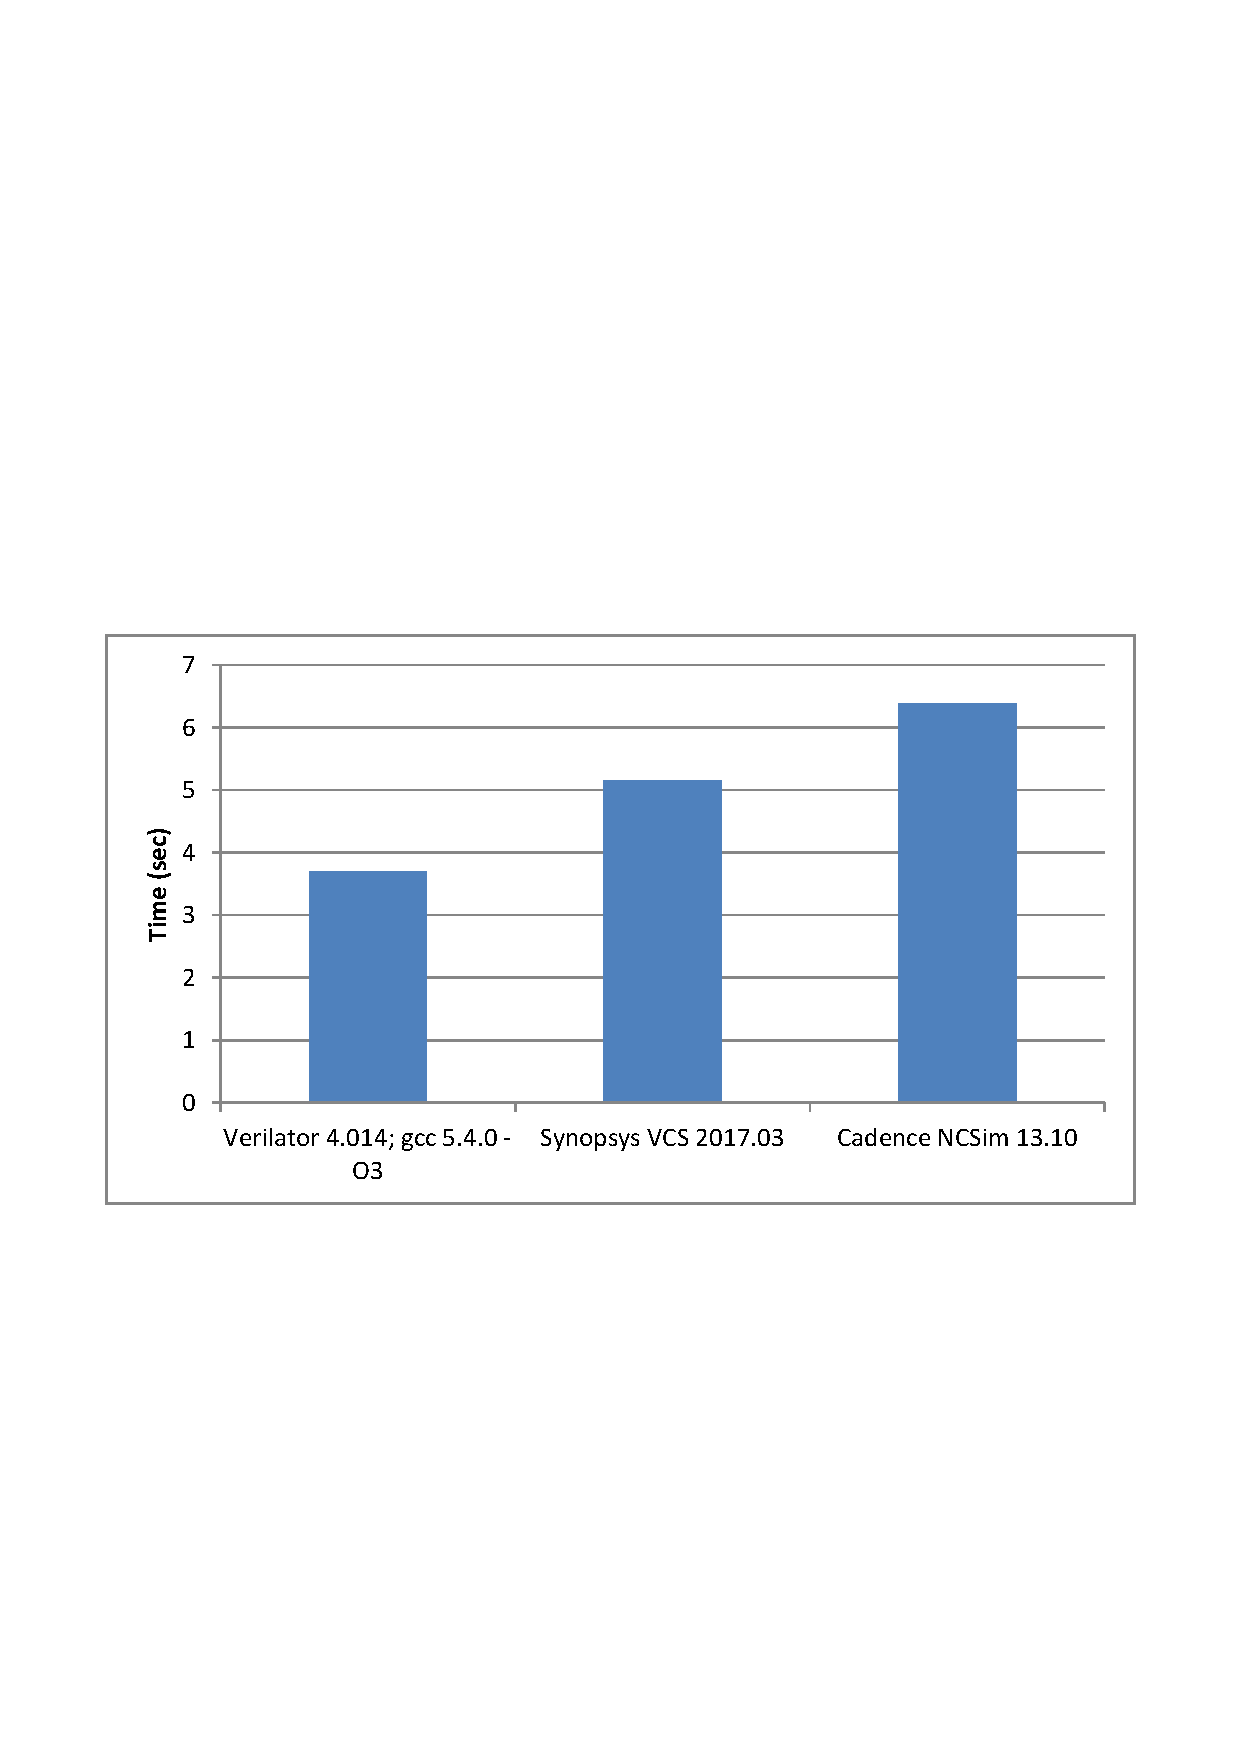
\includegraphics[trim=0 250 0 290 , clip, width=0.93\textwidth]{Figures/benchmark.pdf}
	\caption{RV32-Versat simulation time. Normal mode.}
	\label{fig:benchmark}
\end{figure}

\begin{figure}[!htb]
	\centering
	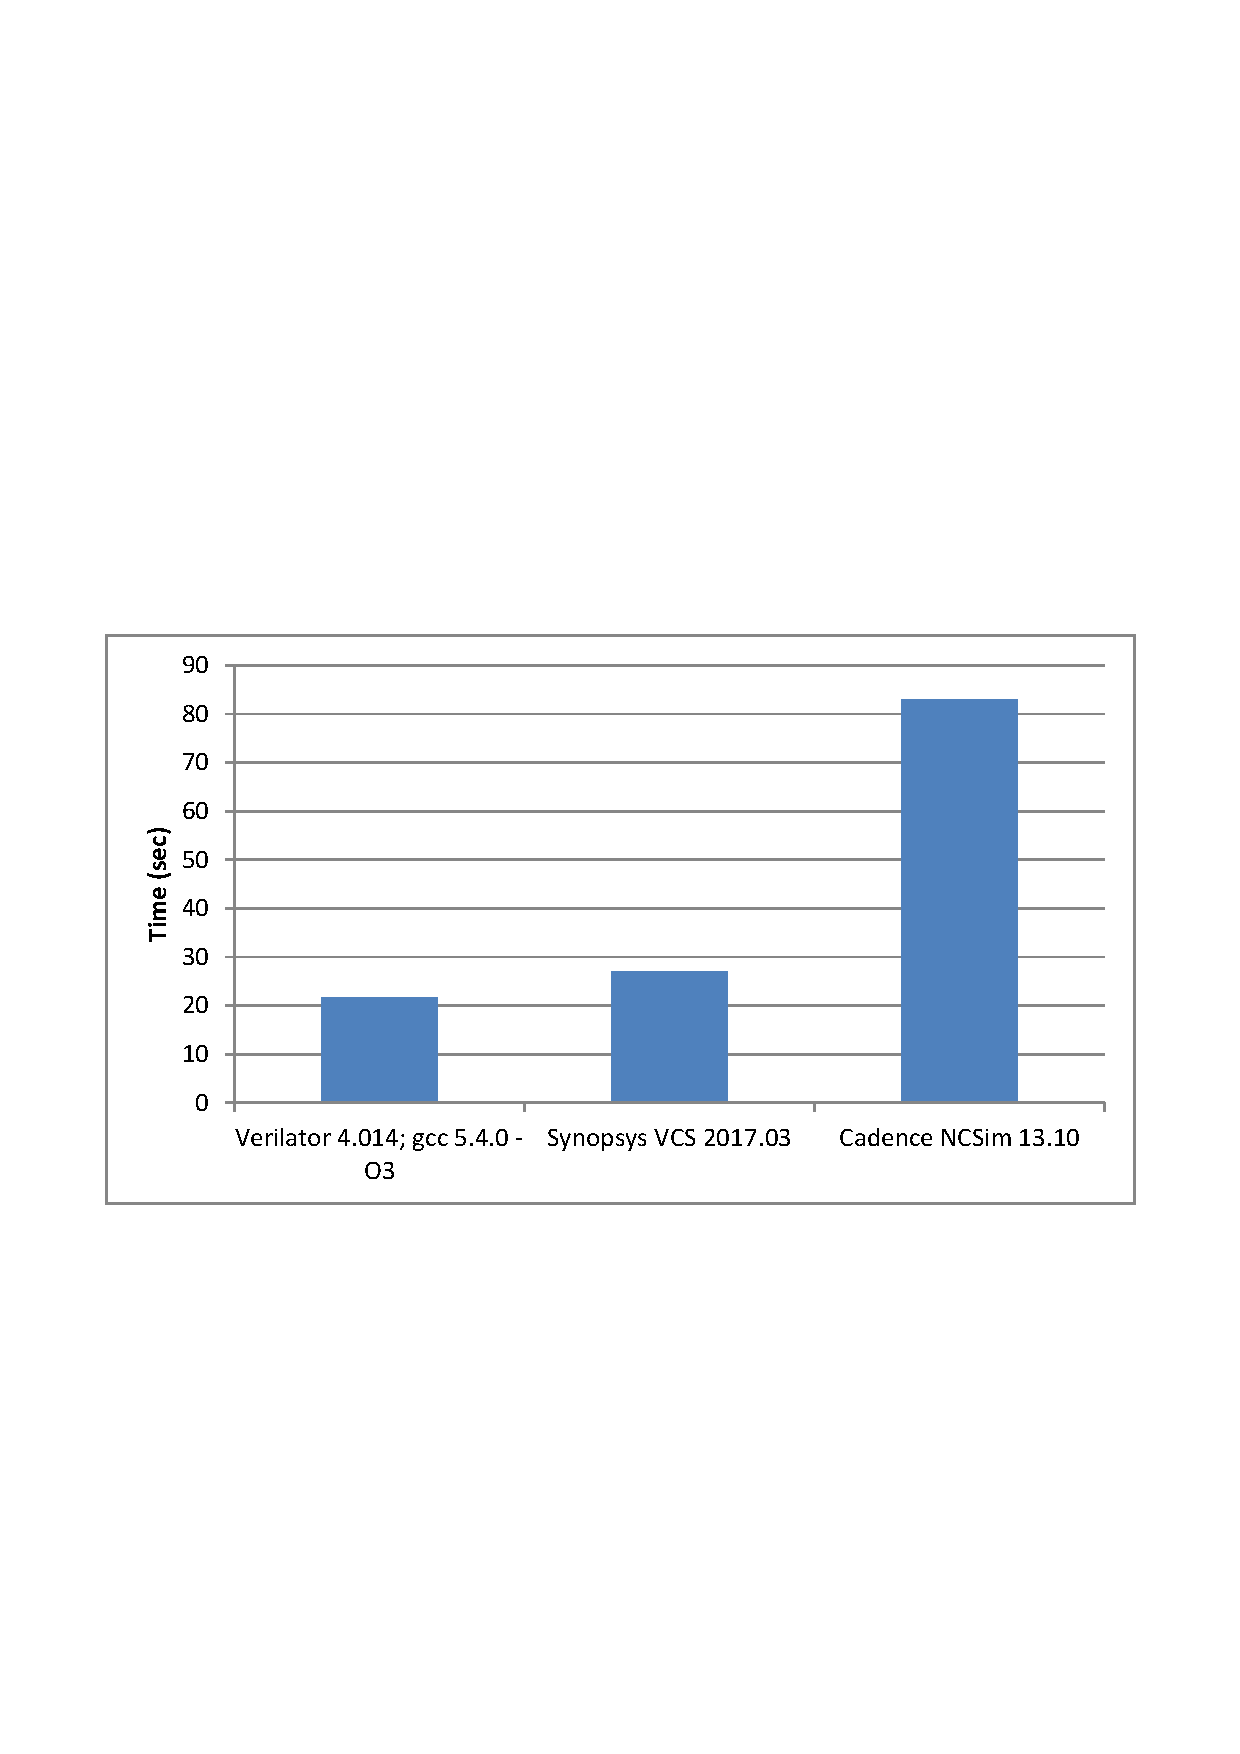
\includegraphics[trim=0 250 0 290 , clip, 
	width=0.93\textwidth]{Figures/benchmark_vcd.pdf}
	\caption{RV32-Versat simulation time. Debug+VCD mode.}
	\label{fig:benchmark_vcd}
\end{figure}

As expected, the simulation times are longer in the debug+\ac{VCD} mode. This happens
because the simulators enable more internal assertions, therefore slowing down
the simulation performance.  Also, the \ac{VCD} file generation further slows down
the simulations, since they have to write a considerable amount of data to the
computer disk. This was probably the main reason for the low performance of
NCsim, since it produced a \ac{VCD} file considerably larger than the other
simulators.

It can be seen that in both tests Verilator is the fastest simulator. This was
expected since Verilator is a cycle-accurate simulator whereas the other two are
event-driven simulators. Event-driven simulators are typically slower since the
algorithms used are more complex than the ones used in cycle-accurate
simulators, as explained in more detail in Section~\ref{section:performance}. The
second fastest simulator was Synopsys VCS, which was 1.39 and 1.24 times slower
than Verilator, for the normal and debug+\ac{VCD} modes, respectively. Finally, the
slowest simulator was Cadence NCSim, 1.73 and 3.81 times slower than
Verilator for the normal and debug+\ac{VCD} modes, respectively. As said before,
event-driven simulators (like Cadence NCSim or Synopsys VCS) provide more
detailed results, being specially useful in the early stages of development or
to simulate individual modules. However, RV32-Versat is a complex system and
each one of its modules has already been vastly tested, so it makes sense to
save time (and money) by using Verilator, since there is a low risk of getting
wrong simulation results due to the simplifications implemented by Verilator.

Comparing the above results with the ones obtained
in~\cite{verilator:benchmarks} and shown in Section~\ref{section:performance},
some differences can be noticed. In spite of Verilator being the fastest
simulator in both results, in this work the difference is smaller. Also, while
in~\cite{verilator:benchmarks} NCSim is the second fastest simulator, here that
does not happen and VCS is faster than NCSim, especially when the debug mode and
\ac{VCD} generation are enabled.

These differences can be caused by multiple factors: the computers used to run
the simulations were different, and the same applies to the simulated models:
in~\cite{verilator:benchmarks} a Motorolla M68K processor derivative was used
whereas here the RV32-Versat system was used. The versions of the simulators
used were also different, and that might be a reason for NCSim being
so slow compared to VCS. In fact, the NCSim version is from 2013. This of course
does not invalidate the results for the present work but it is worth noticing for
the sake of rigour.


\section{FPGA Validation Results}
\label{section:fpga}

The RV32-Versat architecture was implemented in an \ac{FPGA}, more precisely a Xilinx
XCKU040 device of the Kintex UltraScale product family. The whole system was
implemented and tested using the CNN algorithm, previously described in
Section~\ref{section:application}.

The initial values of the Versat memories, which in the simulations were loaded
through the testbench, were now used to initialize the \ac{FPGA} \ac{BRAM} at
compile time, preventing the need to send large quantities of data to the
device. This situation is not ideal, since each time one wants to use a
different set of values, for example, to analyze a different image, the \ac{FPGA}
configuration bit stream needs to be built again, which takes considerable time.

However, in this work the \ac{FPGA} implementation was only used as a way to validate
the simulation results, and further work in this area would be out
of the scope of this dissertation. The simulation results were successfully
validated and the \ac{FPGA} implementation results are presented in 
Table~\ref{tab:resources}, where the amount of \ac{LUT}s, \ac{BRAM}s and \ac{DSP} used 
are shown.

\begin{table}[!htb]
	\renewcommand{\arraystretch}{1.2} % more space between rows
	\caption{FPGA implementation results for RV32-Versat configured for the CNN
		digit recognition application.}
	\label{tab:resources}
	\centering
	\begin{tabular}{llll}
		\toprule
		Resources & LUTs   & BRAMs & DSPs\\
		\midrule
		Used      & 7081   & 62    & 8    \\
		Total     & 242400 & 600   & 1920 \\
		\midrule
		\%        & 2.92   & 10.33 & 0.42 \\
		\bottomrule
	\end{tabular}
\end{table}

%the amount of logic
%used by the RV32-Versat was small given the resources available in the FPGA
%board: only 7081 of the 242400 LUTs (lookup tables) available were used,
%representing 2.92\% of the total available LUTs, at a frequency of operation of
%100 MHz.
